
  AFRP, significa \textit{Arrowized FRP}, es un paradima derivado del
paradigma FRP.

  Otro framework es Yampa \cite{yampa},
un lenguaje embebido en Haskell, que expresa los programas como señales y
define operadores simples para combinarlas y funciones que
procesan las señales.
En Yampa, las señales \ref{fig:arrowcombinators} dejan de ser objetos de primera clase,
y las funciones que las combinan pasan a tomar mayor importancia.

\begin{figure}[h]
\begin{center}
\caption{Combinadores de Yampa}
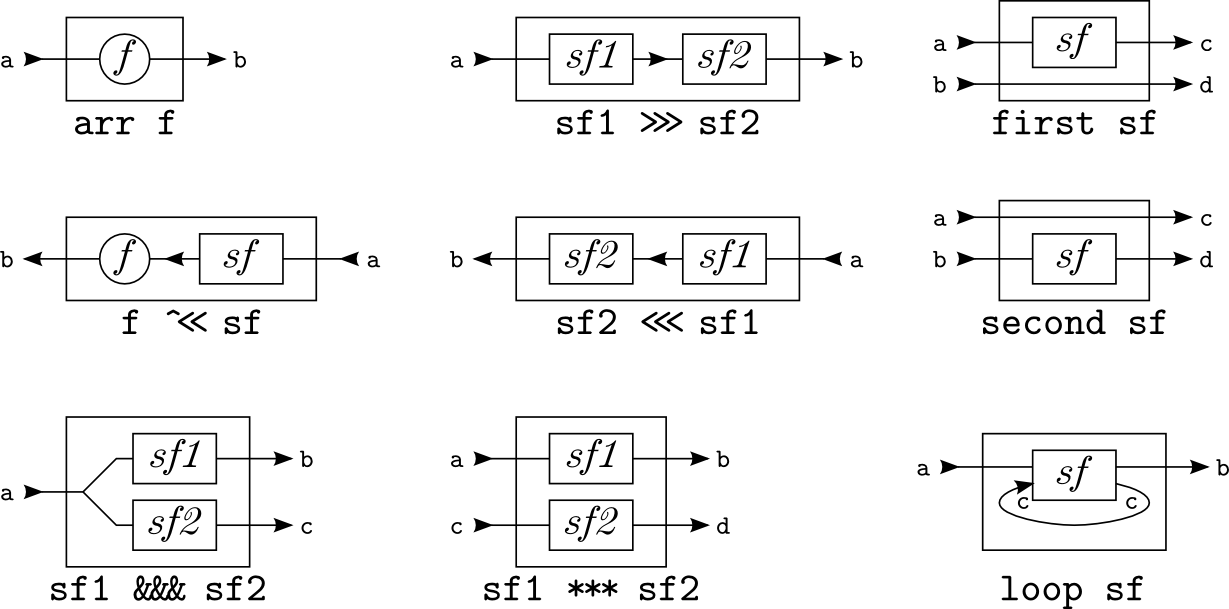
\includegraphics[width=0.9\textwidth]{graphs/yampasf.png}
\label{fig:arrowcombinators}
\end{center}
\end{figure}


